%%%%%%%%%%%%%%%%%%%%%%%%%%%%%%%%%%%%%%%%%%%%%%%%%%%%%%%%%%%%%%%
\section{Production and Assembly}
\label{sec:fdsp-pd-prod-assy}

%%%%PHOTON COLLECTORS PRODUCTION %%%%%%%%%%%%%%%%%%%%%%%%%%%%%%%%%%%%%%%%%%%%%%%%%%%
The \single \dword{pds} consortium is a geographically diverse group of institutions, collaborating across three continents to fabricate a single integrated system.  As such, careful planning and control of component fabrication, assembly and testing must be maintained.
This section describes the planning for fabrication, assembly, and testing, focusing primarily on the \dword{pd} light collector modules, photosensors and photosensor modules, and electronics. It also covers planning for  calibration and monitoring.
 
This section first describes the fabrication procedure for each of the major \dword{pd} system components.  It concludes (in Section~\ref{sec:fdsp-pd-assy-Assby-plan}), by outlining the work flow and responsible institutions for the assembly plan.

%%%%%%%%%%%%%%%%%%%%%%%%%%%%%%%%%%%%%%%
\subsection{Light Collector Module Component Fabrication}

The \dword{pd} light collector modules were designed with ease of fabrication in mind.  The module components can be fabricated and \dword{qc} tested at physically separated facilities, later to be collected and assembled at one or more assembly facilities. 

Each \dword{spmod} detector requires the fabrication of \num{1500} photon detector modules, a significant production effort.  Many of the components for these modules are commercially available or relatively easy to fabricate, but some, such as photosensors (\num{288000} required), filter plates (\num{48000} required), and \dword{wls} plates (\num{6000} required), are specialized items requiring close interfaces with industrial partners.  These issues will be discussed in the relevant sub-sections below.   

%%%%%%%%%%%%%%%%%%%%
\subsubsection{Dichroic Filter and Reflector Foils Fabrication and Coating}

The baseline design for dichroic filters is 
a fused silica plate,  \SI{10}{cm}$\times$\SI{7.8}{cm}$\times$\SI{0.2}{cm}, commercially coated (as described in Section~\ref{sec:fdsp-pd-lc}) to provide the dichroic properties of the filter.  
The filter plates will be purchased from a commercial vendor (certified by the vendor for performance), and the performance of a representative sample will be tested at a collaboration institution as part of our \dword{qc} program.  

Prior to coating, the filters are cleaned using the procedure outlined in Section~\ref{sssec:cleaning}.
For \dword{pd} production, the evaporation process will be performed
in Brazil, where a large vacuum evaporator with an internal diameter of one meter is now available. The conversion efficiency of the film deposited on the filters will be measured for a representative sample, with a dedicated set-up that will use the \SI{127}{nm} light produced by a VUV monochromator.

Vikuiti\texttrademark\ reflector foils required for the rear reflector surface of single-sided X-ARAPUCA supercells and the sides of all modules will be purchased and laser-cut to the form factor required by a vendor.  Mechanical and optical \dword{qc} tests will be performed on a representative sample upon receipt.

Coated filter plates and reflector foils represent one of the more challenging fabrication tasks for the consortium.  A total of \num{48000} filter plates will be required, and fabrication will need to occur at a rate of approximately \num{1200} per month.  Dichroic filters will be purchased as part of the Brazilian effort.  A Brazilian candidate vendor for the filters (Opto Eletronica S.A\footnote{www.opto.com.br}), has been selected for the filter manufacturing.  Preliminary contact has been made, a budgetary estimate received, and initial discussions suggest that they will be capable of meeting our production schedule.  Coating of filter plates will be conducted at \dword{unicamp}.  Prototype studies suggest a coating cycle time of less than two hours per \num{24} filter plates, which meets the needs of the project.

%%%%%%%%%%%%%%%%%%%%
\subsubsection{Wavelength Shifting Plates}

The baseline design for the wavelength-shifting plates are Eljen EJ-286 plates of dimensions \SI{48.7}{cm}$\times$\SI{9.3}{cm}$\times$\SI{0.35}{cm}.  The edges of a plate will be simultaneously cut and polished with a diamond-edged cutter to increase internal reflectivity, following a proprietary process developed by Eljen.  Plates will be delivered to the consortium institution responsible for this component, where \dword{qc} testing of a representative sample will be performed.

Eljen, Inc. has been involved in \dword{pd} module development for many years and has proven a reliable partner.  We have a budgetary estimate for the plates, indicating a total production time of approximately \num{18} months for all \num{6000} wavelength-shifting plates required.

\subsubsection{Mechanical components}

The mechanical components of the \dword{pd} module frames are fabricated from
FR-4 G-10. This material will mitigate thermal expansion issues (see thermal expansion discussion in Section~\ref{sssec:pds-thermal-load}),
but is abrasive and somewhat difficult and expensive to work with using traditional machining processes.

To mitigate these difficulties, most of the \dwords{pd} frame components were designed so that they can be fabricated using water-jet cutting technology.  In some cases, post-cutting fabrication is required, e.g., tapping of pre-cut holes, or (rarely) drilling and tapping holes into the sides of the components where the water jet could not pre-cut pilot holes.

%\fixme{Ettore, Bob--  I changed this text to reflect plans to do water jet cutting in-house}
Water jet cutting of FR-4 G-10 components will be conducted in-house at \dword{unicamp} to allow for improved quality and schedule control.  A dedicated water-jet cutting machine is being purchased now, and fabrication processes will be validated during \dword{sbnd} and \dword{pdsp2} fabrication.  Secondary machining operations (hole tapping, etc.) will also be conducted at \dword{unicamp}.  \dword{qc} tests will be conducted on a representative sample of finished components.

\label{sec:fdsp-pd-prod-pc}

\subsection{Photon Detector Module Assembly}

DUNE \dword{spmod} \dword{pd} module assembly will occur at a \dword{pd} assembly facility at \dword{unicamp}.  Assembly procedures are described below.  Final assembly planning for \dword{pd} modules is guided by the experience gained during the assembly of \num{60} \dword{pdsp} \dword{pd} modules. 


\subsubsection{Incoming Materials Control}

Each \dword{pd} sub-component assembly site will have a quality control supervisor, who will be responsible for overseeing all quality-related activities at that site, maintaining all production records and assembly travelers, and uploading them to the production database as appropriate.   This local supervisor will report directly to the \dword{pd} consortium lead.

All materials for \dword{pd} module assembly will be delivered to the \dword{unicamp} module assembly facility with a \dword{qc} traveler (in the case of materials custom fabricated for DUNE) generated prior to arrival at the assembly site or will have an incoming materials traveler generated immediately upon receipt of the component (for commercial components).  These travelers will be scanned (or uploaded if in electronic format) upon receipt at the assembly facility, and the data stored in the DUNE \dword{qc} database.  Materials will either arrive with a pre-existing DUNE inventory control batch/lot number, or will have one assigned prior to entering the assembly area.  Bar code labels attached to storage containers for all components in the assembly area will facilitate traceability throughout the assembly process.

Immediately upon receipt, all materials will undergo an incoming-materials inspection, including confirmation of key dimensional tolerances as specified on their incoming materials documentation.  
The results of these inspections will be included on the traveler for that batch/lot and entered into the database.

In the case of deviations from specification noted in these inspections, the deviation from nominal will be recorded in an exception section of the traveler, as will the resolution of the discrepancy.

\subsubsection{Assembly Area Requirements}

Assembly will occur in a class \num{100000} or better clean assembly area (see specification SP-PDS-1 in Table \ref{tab:specs:SP-PDS}).  

Photosensitive components (e.g., \dword{tpb}-coated surfaces) are sensitive to near-UV light exposure and will be protected by blue-filtered light in the assembly area (>\SI{400}{nm} or better filters\footnote{For example, GAMTUBE T1510\texttrademark{} from GAM Products, Inc., \url{http://www.gamonline.com/catalog/gamtube/index.php}.}); it has been determined that this level of filtering is sufficient to protect coated surfaces during  exposures of up to several days. For exposures of weeks or months, such as in the ProtoDUNE cryostat assembly area, a higher cutoff yellow filter is used\footnote{F007-010\texttrademark{} Amber with Adhesive - http://www.epakelectronics.com/uv\_filter\_materials\_flexible.htm.}. 

Exposure of photosensitive components will be strictly controlled, per requirement SP-PDS-3 in Table~\ref{tab:specs:SP-PDS}.  
Work flow restrictions will %be restricted to 
ensure no component exceeds a total exposure of \SI{8}{hours} to filtered assembly area lighting (including testing time).

\subsubsection{Component Cleaning}
\label{sssec:cleaning}
All components will be cleaned 
following manufacturer's specifications and DUNE materials test stand recommendations.  
All incoming materials will have written cleaning procedures, and their travelers will document the completion of these procedures.

\subsubsection{Assembly Procedures}

As was done for \dword{pdsp}, detailed step-by-step written procedure documents will 
guide the assembly for each \dword{pd} module, with a \dword{qc} traveler 
completed and recorded in the database.  Travelers will be based on those used for \dword{pdsp}, modified as need to capture additional data needed for \dword{xarapu} module fabrication.

\dword{pdsp} experience suggests that a two-person assembly team is necessary.
Our current assembly plan envisions a pair of two-person assembly teams working simultaneously, with a fifth person acting as shift leader.  This labor force will allow for production of \num{20} \dword{pd} modules per week, meeting our production requirements.  

The shift leader acts as a \dword{qc} officer responsible primarily for ensuring the distribution of materials to the assembly teams, documenting the batch and lot numbers for each \dword{pd} on the travelers, and ensuring that the teams follow the documented assembly procedures.

Assembly fixtures mounted to \SI{2.4}{m} long flat tables will %be used to 
support and align \dword{pd} components during assembly.  All workers handling \dword{pd} components will wear gloves, hair nets, shoe covers, and clean-room disposable laboratory jackets at all times.

\subsubsection{Post-Assembly Quality Control}

Post-assembly \dword{qc} planning is also based on \dword{pdsp} experience, modified as appropriate for larger-scale production.  Each \dword{pd} module goes through a series of ``go-no go'' gauges 
designed to control tolerances of critical interface points.  Following this, each module is inserted into a test \dword{apa} support model, representing the tightest slot allowed by \dword{apa} mechanical tolerances.
It is then scanned at a fixed set of positions with \SI{275}{nm} UV \dwords{led}.  
The \dword{pd} response at each position is measured using \dword{pd} readout electronics and the data compared to reference set of values.
%pre-established criteria.  
Figure~\ref{fig:pds-pd-scanner} shows %is a photograph of 
the scanner used for \dword{pdsp} modules. These performance data will serve as a baseline for the \dword{pd} module, and will be compared against those taken in an identical scanner shortly before installation into an \dword{apa} in the \dword{spmod}, as for \dword{pdsp}. % experience.  
All data collected are recorded to the module traveler and to the DUNE \dword{qc} database.
Post-assembly immersion into a LN2 cryostat followed by a repeat scan of each \dword{pd} module (as in \dword{pdsp}) is under consideration as a final \dword{qc} check.

\begin{dunefigure}[\dshort{pd} module scanner]{fig:pds-pd-scanner}
{\dword{pd} module scanner.}
  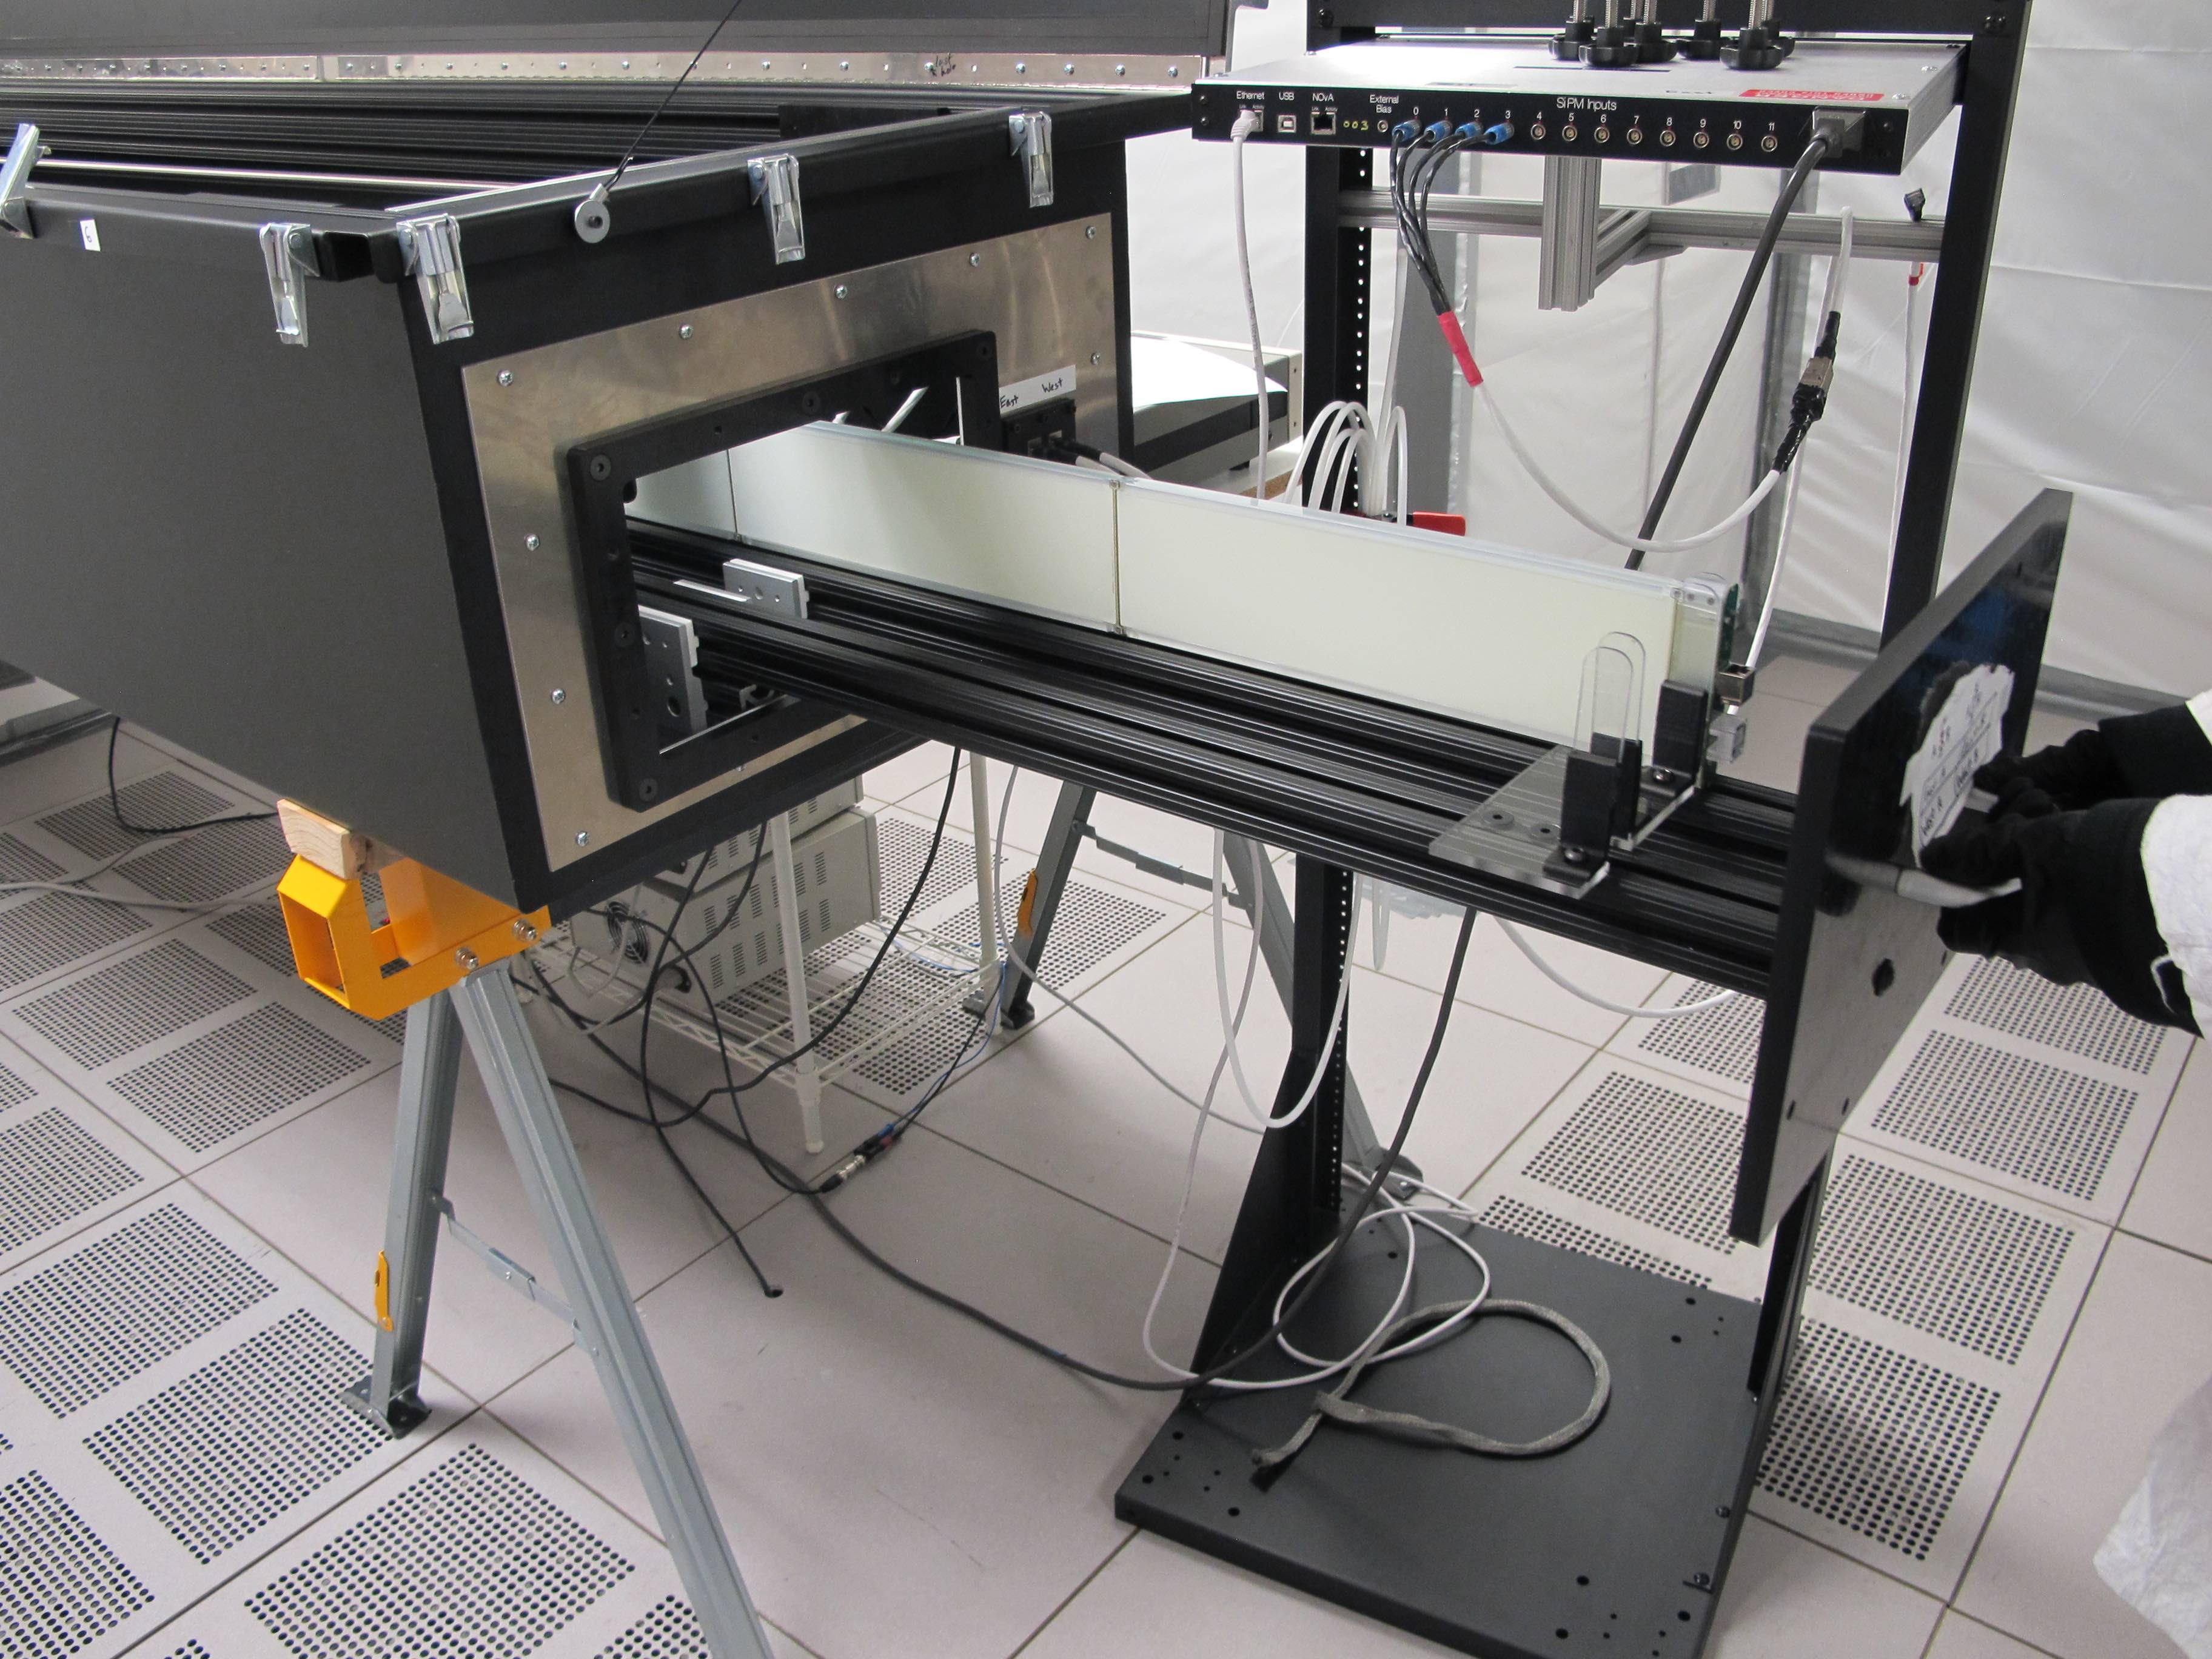
\includegraphics[width=0.5\columnwidth]{pds-pd-scanner.jpg}
\end{dunefigure}


